\documentclass[10pt,a4paper]{extarticle}
\usepackage[a4paper,margin=10mm,top=9mm,bottom=11mm]{geometry}
% ===== Shared preamble: Class 12 Chemistry (project style, from physics-formula-sheet-source.tex) =====
\usepackage[T1]{fontenc}
\usepackage{lmodern}
\usepackage{amsmath,amssymb}
\usepackage{multicol}
\usepackage[most]{tcolorbox}
\usepackage{enumitem}
\usepackage{booktabs,tabularx,array}
\usepackage{fancyhdr}
\usepackage{xcolor}
\usepackage{microtype}
\usepackage[version=4]{mhchem}
\usepackage{tikz}
\usetikzlibrary{arrows.meta,calc}
\usepackage{pifont}
\usepackage{needspace}
\DeclareUnicodeCharacter{21CC}{\ensuremath{\rightleftharpoons}}
\DeclareUnicodeCharacter{2713}{\ding{51}}
\DeclareUnicodeCharacter{03B1}{\ensuremath{\alpha}}
\DeclareUnicodeCharacter{03B2}{\ensuremath{\beta}}
\DeclareUnicodeCharacter{2192}{\ensuremath{\to}}
\DeclareUnicodeCharacter{2610}{\ensuremath{\square}}
\DeclareUnicodeCharacter{21D2}{\ensuremath{\Rightarrow}}
\DeclareUnicodeCharacter{2194}{\ensuremath{\leftrightarrow}}
\DeclareUnicodeCharacter{2605}{\ding{72}}

% ---------- Colours: one per unit ----------
\definecolor{navy}{HTML}{1B2A4A}
\definecolor{uI}{HTML}{1F5FAD}    % 1 Solutions
\definecolor{uII}{HTML}{0E8A7E}   % 2 Electrochemistry
\definecolor{uIII}{HTML}{C2571A}  % 3 Chemical Kinetics
\definecolor{uIV}{HTML}{6A3FA0}   % 4 d- and f-Block
\definecolor{uV}{HTML}{B0204F}    % 5 Coordination Compounds
\definecolor{uVI}{HTML}{2E8B3A}   % 6 Haloalkanes & Haloarenes
\definecolor{uVII}{HTML}{8A6D00}  % 7 Alcohols, Phenols, Ethers
\definecolor{uVIII}{HTML}{2B6F8F} % 8 Aldehydes, Ketones, Acids
\definecolor{uIX}{HTML}{9A4A1E}   % 9 Amines
\definecolor{uX}{HTML}{5A5A5A}    % 10 Biomolecules
\definecolor{tipY}{HTML}{FFF4B8}
\definecolor{tipYframe}{HTML}{E0B400}
\definecolor{sqp}{HTML}{1B2A4A}
\colorlet{uc}{uI}

% ---------- Tag for questions in the official 2026-27 sample paper ----------
\newcommand{\tagbox}[2]{{\setlength{\fboxsep}{0.8pt}\colorbox{#1}{\textcolor{white}{\sffamily\bfseries\tiny\,#2\,}}}}
\newcommand{\SQP}{\tagbox{sqp}{SQP 26--27}}

% ---------- Unit banner & chapter bar ----------
\newcommand{\unitbanner}[3]{% colour, title, marks
  \colorlet{uc}{#1}%
  \par\vspace{2pt}\noindent
  \begin{tcolorbox}[enhanced,colback=#1,colframe=#1,arc=1.5pt,boxsep=1pt,left=4pt,right=4pt,top=1.5pt,bottom=1.5pt,before skip=2pt,after skip=2pt]
  \sffamily\bfseries\color{white}\footnotesize #2\hfill\scriptsize #3
  \end{tcolorbox}}
\newcommand{\chapbar}[1]{%
  \par\needspace{7\baselineskip}\noindent
  \begin{tcolorbox}[enhanced,colback=uc!18,colframe=uc,boxrule=0pt,leftrule=3pt,arc=0pt,boxsep=0.5pt,left=3pt,right=3pt,top=1pt,bottom=1pt,before skip=3pt,after skip=1.5pt]
  \sffamily\bfseries\color{uc!80!black}\footnotesize #1
  \end{tcolorbox}}
\newcommand{\sub}[1]{\par\needspace{4\baselineskip}\addvspace{2pt}\noindent{\sffamily\bfseries\scriptsize\color{uc}\strut\MakeUppercase{#1}}\par\vspace{0.5pt}}

% ---------- Boxes ----------
\newtcolorbox{kbox}{enhanced,colback=uc!5,colframe=uc,boxrule=0.6pt,arc=1.5pt,left=2pt,right=2pt,top=1pt,bottom=1pt,boxsep=1pt,before skip=2pt,after skip=2pt}
\newtcolorbox{tip}{enhanced,colback=tipY,colframe=tipYframe,boxrule=0.5pt,arc=1.5pt,left=2pt,right=2pt,top=0.5pt,bottom=0.5pt,boxsep=1pt,before skip=2pt,after skip=2pt,
  fontupper=\footnotesize}
\newtcolorbox{numbox}{enhanced,colback=white,colframe=uc!70,boxrule=0.5pt,arc=1.5pt,left=2pt,right=2pt,top=0.5pt,bottom=0.5pt,boxsep=1pt,before skip=2pt,after skip=2pt,
  borderline={0.4pt}{1.2pt}{uc!35,dashed}}
\newcommand{\Tip}{{\sffamily\bfseries\scriptsize TIP\;}}
\newcommand{\Num}{{\sffamily\bfseries\scriptsize\color{uc}STANDARD NUMERICALS\;}}

% ---------- Lists ----------
\setlist{nosep,leftmargin=8pt,labelsep=2pt}
\setlist[itemize]{label={\textcolor{uc}{\tiny$\blacktriangleright$}}}
\newenvironment{fl}{\begin{itemize}}{\end{itemize}}

% ---------- Mini graph helper (tikz) ----------
% \minigraph{width}{height}{x label}{y label}{drawing commands}
\newcommand{\minigraph}[5]{%
\begin{tikzpicture}[x=1cm,y=1cm,line cap=round,font=\tiny]
\draw[-{Stealth[length=3pt]},black!70] (0,0)--(#1,0) node[below left,inner sep=1pt]{#3};
\draw[-{Stealth[length=3pt]},black!70] (0,0)--(0,#2) node[above right,inner sep=1pt]{#4};
#5
\end{tikzpicture}}

\setlength{\columnsep}{9pt}
\setlength{\columnseprule}{0.3pt}
\def\columnseprulecolor{\color{black!25}}
\setlength{\parindent}{0pt}
\setlength{\abovedisplayskip}{1pt}\setlength{\belowdisplayskip}{1pt}
\setlength{\abovedisplayshortskip}{0pt}\setlength{\belowdisplayshortskip}{0pt}
\renewcommand{\arraystretch}{1.08}
\newcolumntype{Y}{>{\raggedright\arraybackslash}X}
\pagestyle{fancy}\fancyhf{}
\renewcommand{\headrulewidth}{0pt}

\fancyfoot[L]{\tiny\sffamily\color{black!55} Class 12 Chemistry · \sheetname · CBSE Board 2026--27 (paper 27 Feb 2027)}
\fancyfoot[R]{\tiny\sffamily\color{black!55} Page \thepage}

% ---------- Notes-specific macros ----------
\newcommand{\st}[1]{\textcolor{tipYframe!90!black}{\ifcase#1\or\ding{72}\or\ding{72}\ding{72}\or\ding{72}\ding{72}\ding{72}\fi}}
\newcommand{\ty}[1]{\tagbox{uc!75!black}{#1}}
\newcommand{\mk}[1]{{\scriptsize\color{black!55}[#1]}}
\newenvironment{rqlist}{\begin{enumerate}[leftmargin=12pt,label={\sffamily\bfseries\scriptsize\color{uc}\arabic*.},itemsep=1pt]}{\end{enumerate}}
\newcommand{\ans}{\par\hspace*{2pt}{\color{uc}$\hookrightarrow$}\;}
\newtcolorbox{skel}[1]{enhanced,colback=white,colframe=uc,boxrule=0.5pt,arc=1.5pt,left=3pt,right=3pt,top=1pt,bottom=1pt,boxsep=1pt,before skip=2pt,after skip=3pt,
  title={\sffamily\bfseries\scriptsize #1},colbacktitle=uc!85,coltitle=white,toptitle=0.5pt,bottomtitle=0.5pt}
\newcommand{\chapterhead}[4]{% colour, title, marks, subtitle
  \newpage\colorlet{uc}{#1}%
  \begin{tcolorbox}[enhanced,colback=#1,colframe=#1,arc=2pt,left=6pt,right=6pt,top=3pt,bottom=3pt,after skip=3pt]
  \color{white}\sffamily{\large\bfseries #2}\hfill{\small\bfseries #3}\\[-1pt]{\scriptsize #4}
  \end{tcolorbox}}

% orbital boxes: 0 empty, 1 up, 2 pair, 3 ligand electron pair (shaded)
\newcommand{\ob}[1]{\begin{tikzpicture}[x=2.9mm,y=2.9mm,baseline=0.3mm,line width=0.35pt]
\foreach \s [count=\i from 0] in {#1}{%
 \ifnum\s=3 \fill[uc!28] (\i,0) rectangle ++(1,1);\fi
 \draw[black!65] (\i,0) rectangle ++(1,1);
 \ifnum\s>0 \draw[-{Stealth[length=1.6pt]}] (\i+0.33,0.12)--(\i+0.33,0.88);\fi
 \ifnum\s>1 \draw[{Stealth[length=1.6pt]}-] (\i+0.67,0.12)--(\i+0.67,0.88);\fi}
\end{tikzpicture}}
\def\sheetname{Expert Q\&A}
\raggedbottom
\begin{document}
\small

% ---------- Q&A sheet macros (used after \begin{document}) ----------
\newcounter{qn}\newcounter{an}
\newcommand{\Q}{\par\addvspace{4pt}\refstepcounter{qn}\noindent\hangindent=21pt\hangafter=1\makebox[21pt][l]{\sffamily\bfseries\footnotesize\color{uc}Q\theqn.}}
\newcommand{\An}{\par\addvspace{4pt}\refstepcounter{an}\noindent\hangindent=21pt\hangafter=1\makebox[21pt][l]{\sffamily\bfseries\footnotesize\color{uc}A\thean.}}
\newcommand{\nl}{\par\noindent\hangindent=21pt\hangafter=0}
\newcommand{\secbar}[2]{\par\addvspace{4pt}\needspace{5\baselineskip}\noindent
  \begin{tcolorbox}[enhanced,colback=uc!18,colframe=uc,boxrule=0pt,leftrule=3pt,arc=0pt,boxsep=0.5pt,left=3pt,right=3pt,top=1pt,bottom=1pt,before skip=3pt,after skip=2pt]
  \sffamily\bfseries\color{uc!80!black}\footnotesize #1\hfill\scriptsize #2
  \end{tcolorbox}}
\newcommand{\qatitle}[5]{% number, title, chapters, marks, time
  \gdef\sheetname{Expert Q\&A Sheet #1 of 6: #2}
  \begin{tcolorbox}[enhanced,colback=navy,colframe=navy,arc=2pt,left=8pt,right=8pt,top=5pt,bottom=5pt]
  \color{white}\sffamily
  {\LARGE\bfseries Class 12 Chemistry — Expert Q\&A Sheet #1 of 6}\\[3pt]
  {\large #2} \hfill {\small #3}\\[2pt]
  {\footnotesize CBSE Board 2026--27 pattern · Rationalised NCERT · Paper: \textbf{Sat 27 Feb 2027} · \textbf{#4 marks · #5 min} · Questions first, full-mark answers with step marks at the end}
  \end{tcolorbox}
  \begin{tcolorbox}[enhanced,colback=tipY,colframe=tipYframe,boxrule=0.5pt,arc=1.5pt,left=4pt,right=4pt,top=1.5pt,bottom=1.5pt,before skip=3pt,after skip=3pt]
  \footnotesize\textbf{How to use.} Sit it like a test: set a timer, write on paper, no notes. Then mark yourself against the answer section, step by step. \textbf{Honest label:} every question is \textbf{PYQ-style} — the question types and data patterns that recur in CBSE papers of 2022--2026 and in NCERT — written in my own words, not copied from a specific year's paper. Step-mark splits follow the usual CBSE marking-scheme pattern and are estimates.
  \end{tcolorbox}}
\newcommand{\answerstart}{\newpage
  \begin{tcolorbox}[enhanced,colback=navy,colframe=navy,arc=2pt,left=6pt,right=6pt,top=3pt,bottom=3pt,after skip=3pt]
  \color{white}\sffamily{\large\bfseries Answers \& marking scheme}\hfill{\small written the way a full-marks script reads · {\scriptsize[\,]} = step marks}
  \end{tcolorbox}}
\newcommand{\scorebox}[1]{%
  \begin{tcolorbox}[enhanced,colback=white,colframe=navy,boxrule=0.8pt,arc=2pt,title={\sffamily\bfseries\footnotesize My score: \underline{\hspace{10mm}} / #1 \quad · \quad Time taken: \underline{\hspace{10mm}} min \quad · \quad Questions to redo / errors to log},colbacktitle=navy,coltitle=white,height fill,before skip=4pt]
  \end{tcolorbox}}

\colorlet{uc}{uV}
\qatitle{2}{Inorganic Chemistry}{Ch 4 The d- and f-Block Elements · Ch 5 Coordination Compounds}{42}{75}
\begin{multicols}{2}\raggedcolumns
\secbar{SECTION A · MCQ and assertion--reason}{8 × 1 = 8}
\Q Which ion has the largest number of unpaired electrons?\nl (a) Ti$^{3+}$ \quad (b) Cr$^{3+}$ \quad (c) Mn$^{2+}$ \quad (d) Ni$^{2+}$ \mk{1}
\Q Which ion is colourless in aqueous solution?\nl (a) Sc$^{3+}$ \quad (b) Ti$^{3+}$ \quad (c) V$^{3+}$ \quad (d) Cu$^{2+}$ \mk{1}
\Q The coordination number of cobalt in \ce{[CoCl2(en)2]+} is\nl (a) 2 \quad (b) 4 \quad (c) 5 \quad (d) 6 \mk{1}
\Q The number of ions given by one formula unit of \ce{K4[Fe(CN)6]} in water is\nl (a) 2 \quad (b) 5 \quad (c) 10 \quad (d) 11 \mk{1}
\Q Which complex can show linkage isomerism?\nl (a) \ce{[Co(NH3)6]Cl3} \quad (b) \ce{[Co(NH3)5(NO2)]Cl2}\nl (c) \ce{[Co(NH3)5Cl]SO4} \quad (d) \ce{[Cr(H2O)6]Cl3} \mk{1}
\Q In acidic medium, the number of moles of \ce{Fe^2+} oxidised by one mole of \ce{KMnO4} is\nl (a) 1 \quad (b) 3 \quad (c) 5 \quad (d) 6 \mk{1}
\nl\textit{For Q7--Q8 choose: (a) A and R true, R explains A; (b) both true, R does not explain A; (c) A true, R false; (d) A false, R true.}
\Q \textbf{A:} Zr and Hf have almost identical atomic radii. \textbf{R:} Lanthanoid contraction offsets the expected increase in size from the 4d to the 5d series. \mk{1}
\Q \textbf{A:} \ce{[Ni(CN)4]^2-} is diamagnetic. \textbf{R:} \ce{CN-} is a weak-field ligand. \mk{1}

\secbar{SECTION B · Very short answer}{4 × 2 = 8}
\Q Give reasons: (i) zinc is not regarded as a transition element; (ii) \ce{Cr^2+} is a strong reducing agent. \mk{2}
\Q Complete and balance (acidic medium):\nl (i) \ce{MnO4- + C2O4^2- + H+ ->} \quad (ii) \ce{Cr2O7^2- + Fe^2+ + H+ ->} \mk{2}
\Q Write the IUPAC names of (i) \ce{[CoCl(NH3)5]Cl2} and (ii) \ce{K3[Fe(C2O4)3]}. \mk{2}
\Q Draw the geometrical isomers of \ce{[Pt(NH3)2Cl2]}. Which one is used in cancer treatment? \mk{2}

\secbar{SECTION C · Short answer}{4 × 3 = 12}
\Q What is lanthanoid contraction? State its cause and two consequences. \mk{3}
\Q Give reasons:\nl (i) Transition metals form coloured compounds.\nl (ii) $E^\circ$ for \ce{Mn^3+/Mn^2+} (+1.57 V) is much more positive than for \ce{Fe^3+/Fe^2+} (+0.77 V).\nl (iii) Actinoids show a wider range of oxidation states than lanthanoids. \mk{3}
\Q Using valence bond theory, give the hybridisation, shape and magnetic character of \ce{[CoF6]^3-} and \ce{[Co(NH3)6]^3+}. Which is the inner-orbital complex? (Co: Z = 27) \mk{3}
\Q (a) Write the formula of tetraamminediaquacobalt(III) chloride.\nl (b) Write the electronic configuration of a $d^4$ ion in an octahedral field when (i) $\Delta_o>P$, (ii) $\Delta_o<P$.\nl (c) Why are low-spin tetrahedral complexes rarely observed? \mk{3}

\secbar{SECTION D · Case-based}{1 × 4 = 4}
\Q \textit{In a complex the ligands split the d orbitals of the metal into two sets. In an octahedral field the gap is $\Delta_o$. An electron can jump from the lower to the upper set by absorbing light; if this falls in the visible region, the complex shows the complementary colour. The size of $\Delta_o$ depends on the ligand, so the same metal ion can show different colours with different ligands.}\\[2pt]
(i) Why is \ce{[Ti(H2O)6]^3+} coloured while \ce{[Sc(H2O)6]^3+} is colourless? \mk{1}\\
(ii) Arrange \ce{H2O}, \ce{CN-}, \ce{Cl-}, \ce{NH3} in increasing order of field strength. \mk{1}\\
(iii) Why do dilute solutions of \ce{[Fe(CN)6]^4-} and \ce{[Fe(H2O)6]^2+} have different colours? \mk{2}\\
\textbf{OR} (iii) Write the $t_{2g}$/$e_g$ configuration and number of unpaired electrons in \ce{[Fe(CN)6]^4-} and \ce{[Fe(H2O)6]^2+}. \mk{2}

\secbar{SECTION E · Long answer}{2 × 5 = 10}
\Q (a) Describe, with equations, the preparation of \ce{KMnO4} from pyrolusite ore (\ce{MnO2}). \mk{2}\\
(b) Calculate the spin-only magnetic moment of \ce{Cr^3+} (Z = 24). \mk{1}\\
(c) Give reasons: (i) \ce{Cu+} is unstable in aqueous solution; (ii) the highest oxidation state of a transition metal is shown in its oxides and oxoanions. \mk{2}
\Q (a) \ce{[NiCl4]^2-} is paramagnetic but \ce{[Ni(CO)4]} is diamagnetic, though both are tetrahedral. Explain. (Ni: Z = 28) \mk{2}\\
(b) How many stereoisomers does \ce{[CoCl2(en)2]+} have? Describe them and say which are optically active. \mk{2}\\
(c) Name the isomerism shown by \ce{[Co(NH3)5(SO4)]Br} and \ce{[Co(NH3)5Br]SO4}, and give a test to tell them apart. \mk{1}
\end{multicols}

\answerstart
\begin{multicols}{2}\raggedcolumns
\secbar{SECTION A}{1 mark each}
\An \textbf{(c) Mn$^{2+}$.} $3d^5$: 5 unpaired (Ti$^{3+}$ 1, Cr$^{3+}$ 3, Ni$^{2+}$ 2).
\An \textbf{(a) Sc$^{3+}$.} $3d^0$: no d--d transition possible.
\An \textbf{(d) 6.} en is didentate: $2\times2+2=6$ donor atoms.
\An \textbf{(b) 5.} \ce{K4[Fe(CN)6] -> 4K+ + [Fe(CN)6]^4-}.
\An \textbf{(b).} \ce{NO2-} is ambidentate (binds through N or O).
\An \textbf{(c) 5.} \ce{MnO4- + 5Fe^2+ + 8H+ -> Mn^2+ + 5Fe^3+ + 4H2O}.
\An \textbf{(a).}
\An \textbf{(c).} \ce{CN-} is a \emph{strong}-field ligand; it pairs the $3d^8$ electrons ($dsp^2$, no unpaired electron).

\secbar{SECTION B}{2 marks each}
\An (i) Zn is [Ar]$3d^{10}4s^2$; its d subshell is completely filled in the atom and in \ce{Zn^2+} ($3d^{10}$), so it has no partly filled d orbitals in any common oxidation state. \mk{1}\nl
(ii) \ce{Cr^2+} ($3d^4$) changes to \ce{Cr^3+} ($3d^3$), which has the stable half-filled $t_{2g}^3$ configuration; hence $E^\circ_{\ce{Cr^3+/Cr^2+}}$ is negative ($-0.41$ V) and \ce{Cr^2+} readily loses an electron. \mk{1}
\An (i) \ce{2MnO4- + 5C2O4^2- + 16H+ -> 2Mn^2+ + 10CO2 + 8H2O} \mk{1}\nl
(ii) \ce{Cr2O7^2- + 6Fe^2+ + 14H+ -> 2Cr^3+ + 6Fe^3+ + 7H2O} \mk{1}
\An (i) pentaamminechloridocobalt(III) chloride \mk{1}\nl (ii) potassium trioxalatoferrate(III) \mk{1}
\An \begin{minipage}[t]{0.5\linewidth}\vspace{0pt}
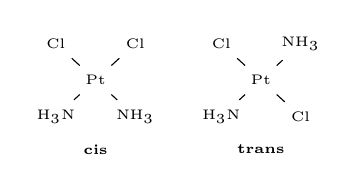
\begin{tikzpicture}[x=4.2mm,y=4.2mm,font=\tiny]
\node (p) at (0,0){Pt}; \node (a) at (-1.2,1.1){Cl}; \node (b) at (1.2,1.1){Cl}; \node (c) at (-1.2,-1.1){H$_3$N}; \node (d) at (1.2,-1.1){NH$_3$};
\foreach \n in {a,b,c,d}{\draw (p)--(\n);} \node at (0,-2.1){\textbf{cis}};
\begin{scope}[xshift=21mm]
\node (p) at (0,0){Pt}; \node (a) at (-1.2,1.1){Cl}; \node (b) at (1.2,1.1){NH$_3$}; \node (c) at (-1.2,-1.1){H$_3$N}; \node (d) at (1.2,-1.1){Cl};
\foreach \n in {a,b,c,d}{\draw (p)--(\n);} \node at (0,-2.1){\textbf{trans}};
\end{scope}
\end{tikzpicture}\end{minipage}\hfill
\begin{minipage}[t]{0.46\linewidth}\vspace{0pt}
Square planar: \emph{cis} has the two Cl adjacent (90$^\circ$); \emph{trans} has them opposite (180$^\circ$). \mk{½ + ½}\\
The \textbf{cis} isomer (cis-platin) is the anticancer drug. \mk{1}
\end{minipage}

\secbar{SECTION C}{3 marks each}
\An \textbf{Lanthanoid contraction} is the steady decrease in atomic and ionic radii of the lanthanoids from La to Lu. \mk{1}\nl
\textbf{Cause:} the 4f electrons shield one another from the nucleus very poorly, so the effective nuclear charge rises with atomic number. \mk{1}\nl
\textbf{Consequences:} (i) 4d and 5d elements of a group have almost the same radii (Zr 160 pm, Hf 159 pm), so they occur together and are hard to separate; (ii) basic strength of the hydroxides decreases from \ce{La(OH)3} to \ce{Lu(OH)3}. \mk{½ + ½}
\An (i) Their ions have partly filled d orbitals; visible light is absorbed for d--d transitions and the complementary colour is seen. \mk{1}\nl
(ii) \ce{Mn^2+} is $3d^5$ (half-filled, extra stable), so \ce{Mn^3+} ($3d^4$) is easily reduced to it. \ce{Fe^3+} is itself $3d^5$, so it is much less ready to be reduced to \ce{Fe^2+} ($3d^6$). \mk{1}\nl
(iii) In actinoids the 5f, 6d and 7s levels have comparable energies, so more electrons can take part in bonding. \mk{1}
\An \ce{Co^3+}: [Ar]$3d^6$.\nl
\ce{[CoF6]^3-}: \ce{F-} is a weak-field ligand, no pairing.\nl \ob{2,1,1,1,1}\,\ob{3}\,\ob{3,3,3}\,\ob{3,3,0,0,0} {\tiny(3d | 4s | 4p | 4d)}\nl
\textbf{$sp^3d^2$}, octahedral, \textbf{paramagnetic} (4 unpaired electrons); outer-orbital (high-spin) complex. \mk{1½}\nl
\ce{[Co(NH3)6]^3+}: \ce{NH3} causes pairing of the 3d electrons.\nl \ob{2,2,2,3,3}\,\ob{3}\,\ob{3,3,3} {\tiny(3d | 4s | 4p)}\nl
\textbf{$d^2sp^3$}, octahedral, \textbf{diamagnetic}; this is the \textbf{inner-orbital} (low-spin) complex. \mk{1½}
\An (a) \ce{[Co(NH3)4(H2O)2]Cl3} \mk{1}\nl
(b) (i) $\Delta_o>P$ (strong field): $t_{2g}^4e_g^0$; (ii) $\Delta_o<P$ (weak field): $t_{2g}^3e_g^1$. \mk{½ + ½}\nl
(c) The tetrahedral splitting is small, $\Delta_t=\frac49\Delta_o$, and is less than the pairing energy, so electrons occupy the higher orbitals rather than pair. \mk{1}

\secbar{SECTION D}{4 marks}
\An (i) \ce{Ti^3+} is $3d^1$: the electron is excited from $t_{2g}$ to $e_g$ by absorbing visible light (d--d transition). \ce{Sc^3+} is $3d^0$: no d electron, no transition. \mk{1}\nl
(ii) \ce{Cl-} $<$ \ce{H2O} $<$ \ce{NH3} $<$ \ce{CN-} \mk{1}\nl
(iii) \ce{CN-} is a strong-field ligand and gives a large $\Delta_o$; \ce{H2O} is weak-field and gives a small $\Delta_o$. \mk{1} The two complexes therefore absorb light of different wavelengths and transmit different complementary colours. \mk{1}\nl
\textbf{OR} (iii) \ce{Fe^2+} is $3d^6$. \ce{[Fe(CN)6]^4-}: $t_{2g}^6e_g^0$, no unpaired electron. \mk{1} \ce{[Fe(H2O)6]^2+}: $t_{2g}^4e_g^2$, 4 unpaired electrons. \mk{1}

\secbar{SECTION E}{5 marks each}
\An (a) \ce{MnO2} is fused with KOH in the presence of air (or an oxidising agent such as \ce{KNO3}) to give green potassium manganate:\nl
\ce{2MnO2 + 4KOH + O2 -> 2K2MnO4 + 2H2O} \mk{1}\nl
Manganate disproportionates in neutral or acidic solution to give purple permanganate:\nl
\ce{3MnO4^2- + 4H+ -> 2MnO4- + MnO2 + 2H2O} \mk{1}\nl
(b) \ce{Cr^3+}: [Ar]$3d^3$, $n=3$; $\mu=\sqrt{n(n+2)}=\sqrt{15}=\boxed{3.87\text{ BM}}$ \mk{1}\nl
(c)(i) \ce{Cu+} disproportionates: \ce{2Cu+(aq) -> Cu^2+(aq) + Cu(s)}. The much more negative hydration enthalpy of \ce{Cu^2+} more than compensates for the second ionisation enthalpy of Cu. \mk{1}\nl
(ii) Oxygen is small and highly electronegative and can form multiple bonds with the metal, which stabilises high oxidation states (e.g.\ Mn(VII) in \ce{MnO4-}). \mk{1}
\An (a) \ce{[NiCl4]^2-}: \ce{Ni^2+} is $3d^8$; \ce{Cl-} is a weak-field ligand, so no pairing; $sp^3$; two unpaired electrons ⇒ paramagnetic. \mk{1}\nl
\ce{[Ni(CO)4]}: Ni(0) is $3d^84s^2$; CO is a strong-field ligand and pushes the 4s electrons into 3d ($3d^{10}$); $sp^3$; no unpaired electron ⇒ diamagnetic. \mk{1}\nl
(b) \textbf{Three} stereoisomers. \emph{trans} (the two Cl at 180$^\circ$): has a plane of symmetry, optically inactive. \emph{cis} (the two Cl at 90$^\circ$): exists as a pair of non-superimposable mirror images, $d$ and $l$, both optically active. \mk{2}\nl
(c) \textbf{Ionisation isomerism.} \ce{[Co(NH3)5Br]SO4} gives a white precipitate (\ce{BaSO4}) with \ce{BaCl2} solution; \ce{[Co(NH3)5(SO4)]Br} gives a pale yellow precipitate (AgBr) with \ce{AgNO3} solution. \mk{1}
\end{multicols}
\begin{tcolorbox}[enhanced,colback=tipY,colframe=tipYframe,boxrule=0.5pt,arc=1.5pt,left=4pt,right=4pt,top=2pt,bottom=2pt,before skip=4pt]
\footnotesize\textbf{Where a 70/70 script wins marks here.} (1) Configurations are always written before the reason (``\ce{Mn^2+} is $3d^5$, so …''). (2) Ionic equations are checked for charge on both sides. (3) VBT answers follow one chain: oxidation state → $d^n$ → strong/weak ligand → box diagram → hybridisation → shape → magnetism. (4) Names are spelt exactly: ammine, chlorido, -ate, Roman numeral, no space inside the complex. (5) For isomers, say \emph{why} one is optically inactive (plane of symmetry). In the exam, draw the octahedra for Q19(b); the drawing carries the marks.
\end{tcolorbox}
\scorebox{42}

\end{document}
